%% using aastex version 6.31
\documentclass[twocolumn]{aastex631}
\usepackage{CJK}
% \usepackage{lineno}
% \linenumbers

\newcommand{\sn}{SN\,2022joj}
\newcommand{\trmax}{$t_{r_\mathrm{ZTF},\mathrm{max}}$}
\newcommand{\tfl}{$t_\mathrm{fl}$}
\newcommand{\Mch}{$M_\mathrm{Ch}$}
\newcommand{\kms}{$\mathrm{km}\,\mathrm{s}^{-1}$}
\newcommand{\Ni}{$^{56}\mathrm{Ni}$}
\newcommand{\Msun}{\mathrm{M_\odot}}
\newcommand{\adam}[1]{\textcolor{red}{[AAM: #1]}}
\newcommand{\chang}[1]{\textcolor{blue}{[Chang: #1]}}

\shorttitle{\sn}
\shortauthors{Liu et al.}
\graphicspath{{./}{figures/}}


\begin{document}
\begin{CJK*}{UTF8}{gbsn}

\title{SN\,2022joj}

%main contributors
\author[0000-0002-7866-4531]{Chang~Liu}
\affil{Department of Physics and Astronomy, Northwestern University, 2145 Sheridan Rd, Evanston, IL 60208, USA}
\affil{Center for Interdisciplinary Exploration and Research in Astrophysics (CIERA), Northwestern University, 1800 Sherman Ave, Evanston, IL 60201, USA}

\author[0000-0001-9515-478X]{Adam~A.~Miller}
\affil{Department of Physics and Astronomy, Northwestern University, 2145 Sheridan Rd, Evanston, IL 60208, USA}
\affil{Center for Interdisciplinary Exploration and Research in Astrophysics (CIERA), Northwestern University, 1800 Sherman Ave, Evanston, IL 60201, USA}

\author{Friends}
\begin{abstract} 
%

%
\end{abstract}

\keywords{Supernovae (1668), Type Ia supernovae (1728), White dwarf stars (1799), Observational astronomy (1145), Surveys (1671)}

\section{Introduction} \label{sec:intro}\section{Observations} \label{sec:obs}
\subsection{Optical Photometry}
\begin{figure*}
    \centering
    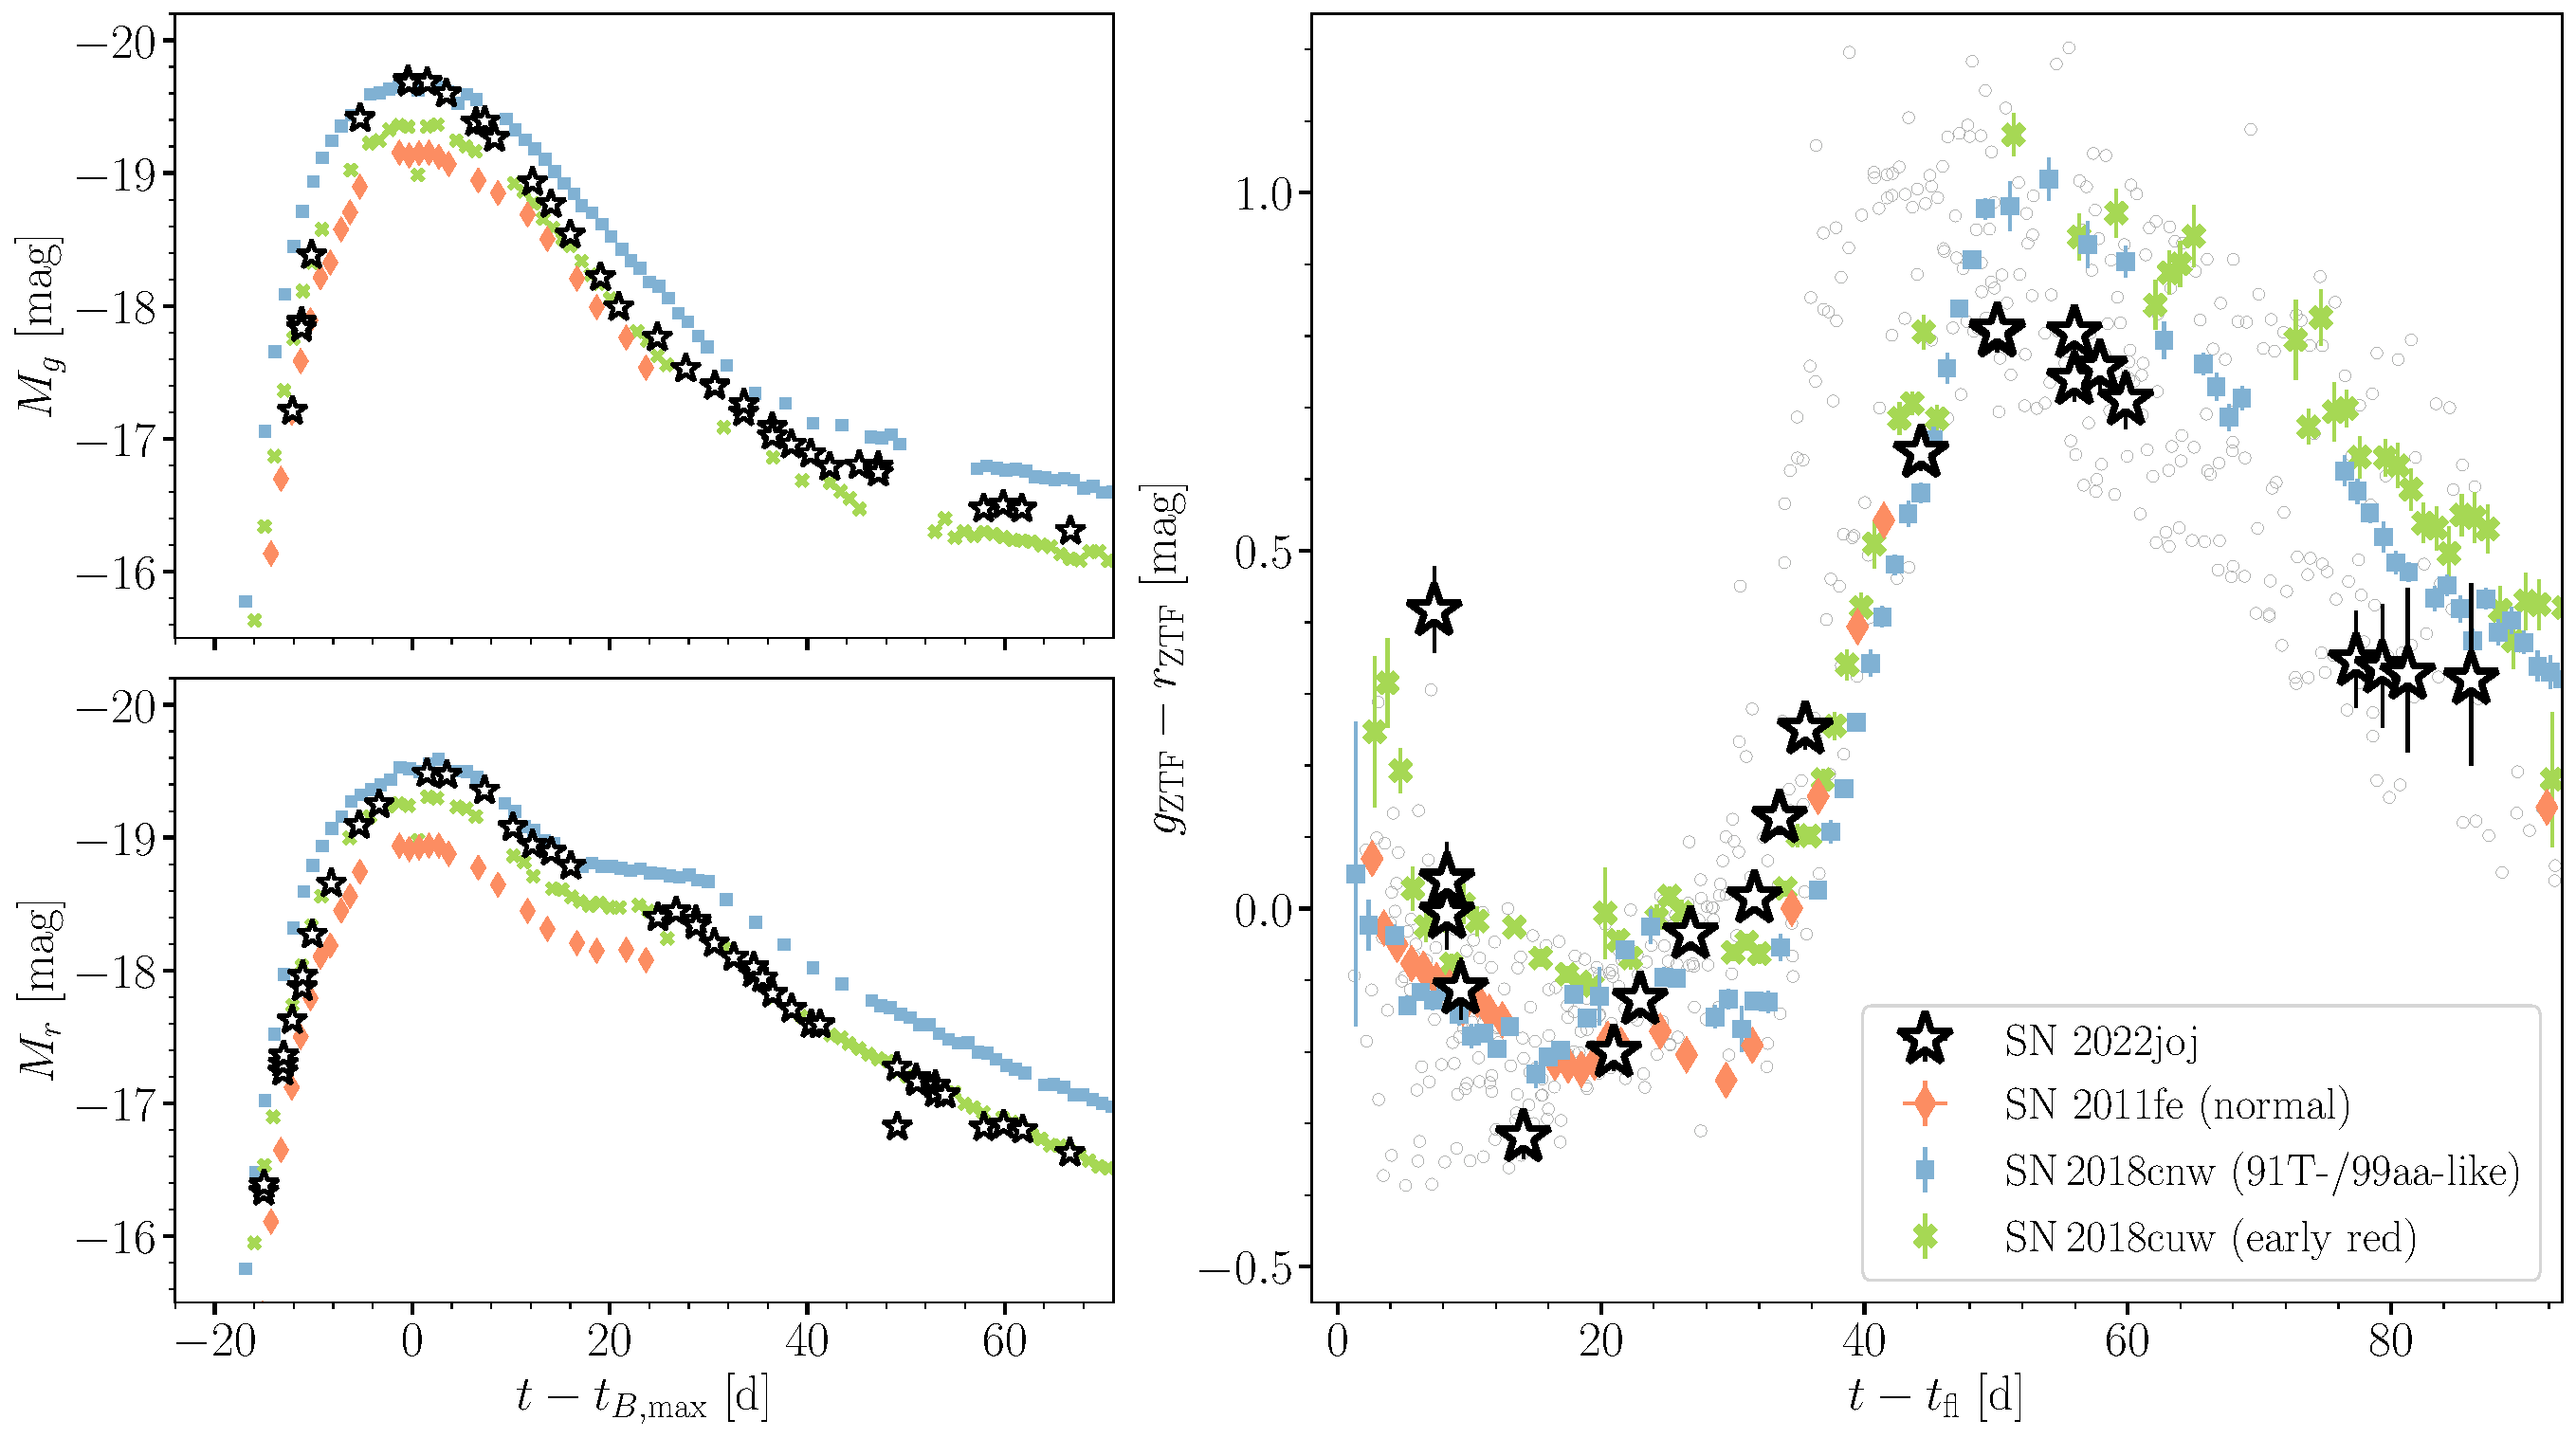
\includegraphics[width=\textwidth]{photometry.pdf}
    \label{fig:lc}
    \caption{Comparison of the photometric properties of \sn\ with those of ZTF18abauprj (99aa-/91T-like SN) and SN\,2013bh (00cx-like SN). \textit{Left}: multiband light curves. The upper (lower) panel shows the evolution in the $g$-band ($r$-band) absolute magnitude. %{The arrows mark the 5$\sigma$ limit of the last nondetections of \sn\ in $g_\mathrm{ZTF}$ and $r_\mathrm{ZTF}$.} 
    \textit{Right}: $g-r$ color evolution. %For each object, the peak epoch is marked by a vertical line with the corresponding color on the bottom axis. 
    The gray circles denote the $g_\mathrm{ZTF}-r_\mathrm{ZTF}$ color evolution of 12 nearby ($z\le0.05$) normal SNe\,Ia (open circles) from the ZTF sample with prompt observations within 5\,days of first light \citep{Bulla2020}.}
\end{figure*}
\subsection{Optical Spectroscopy}\label{sec:optical_spec}
\begin{figure}
    \centering
    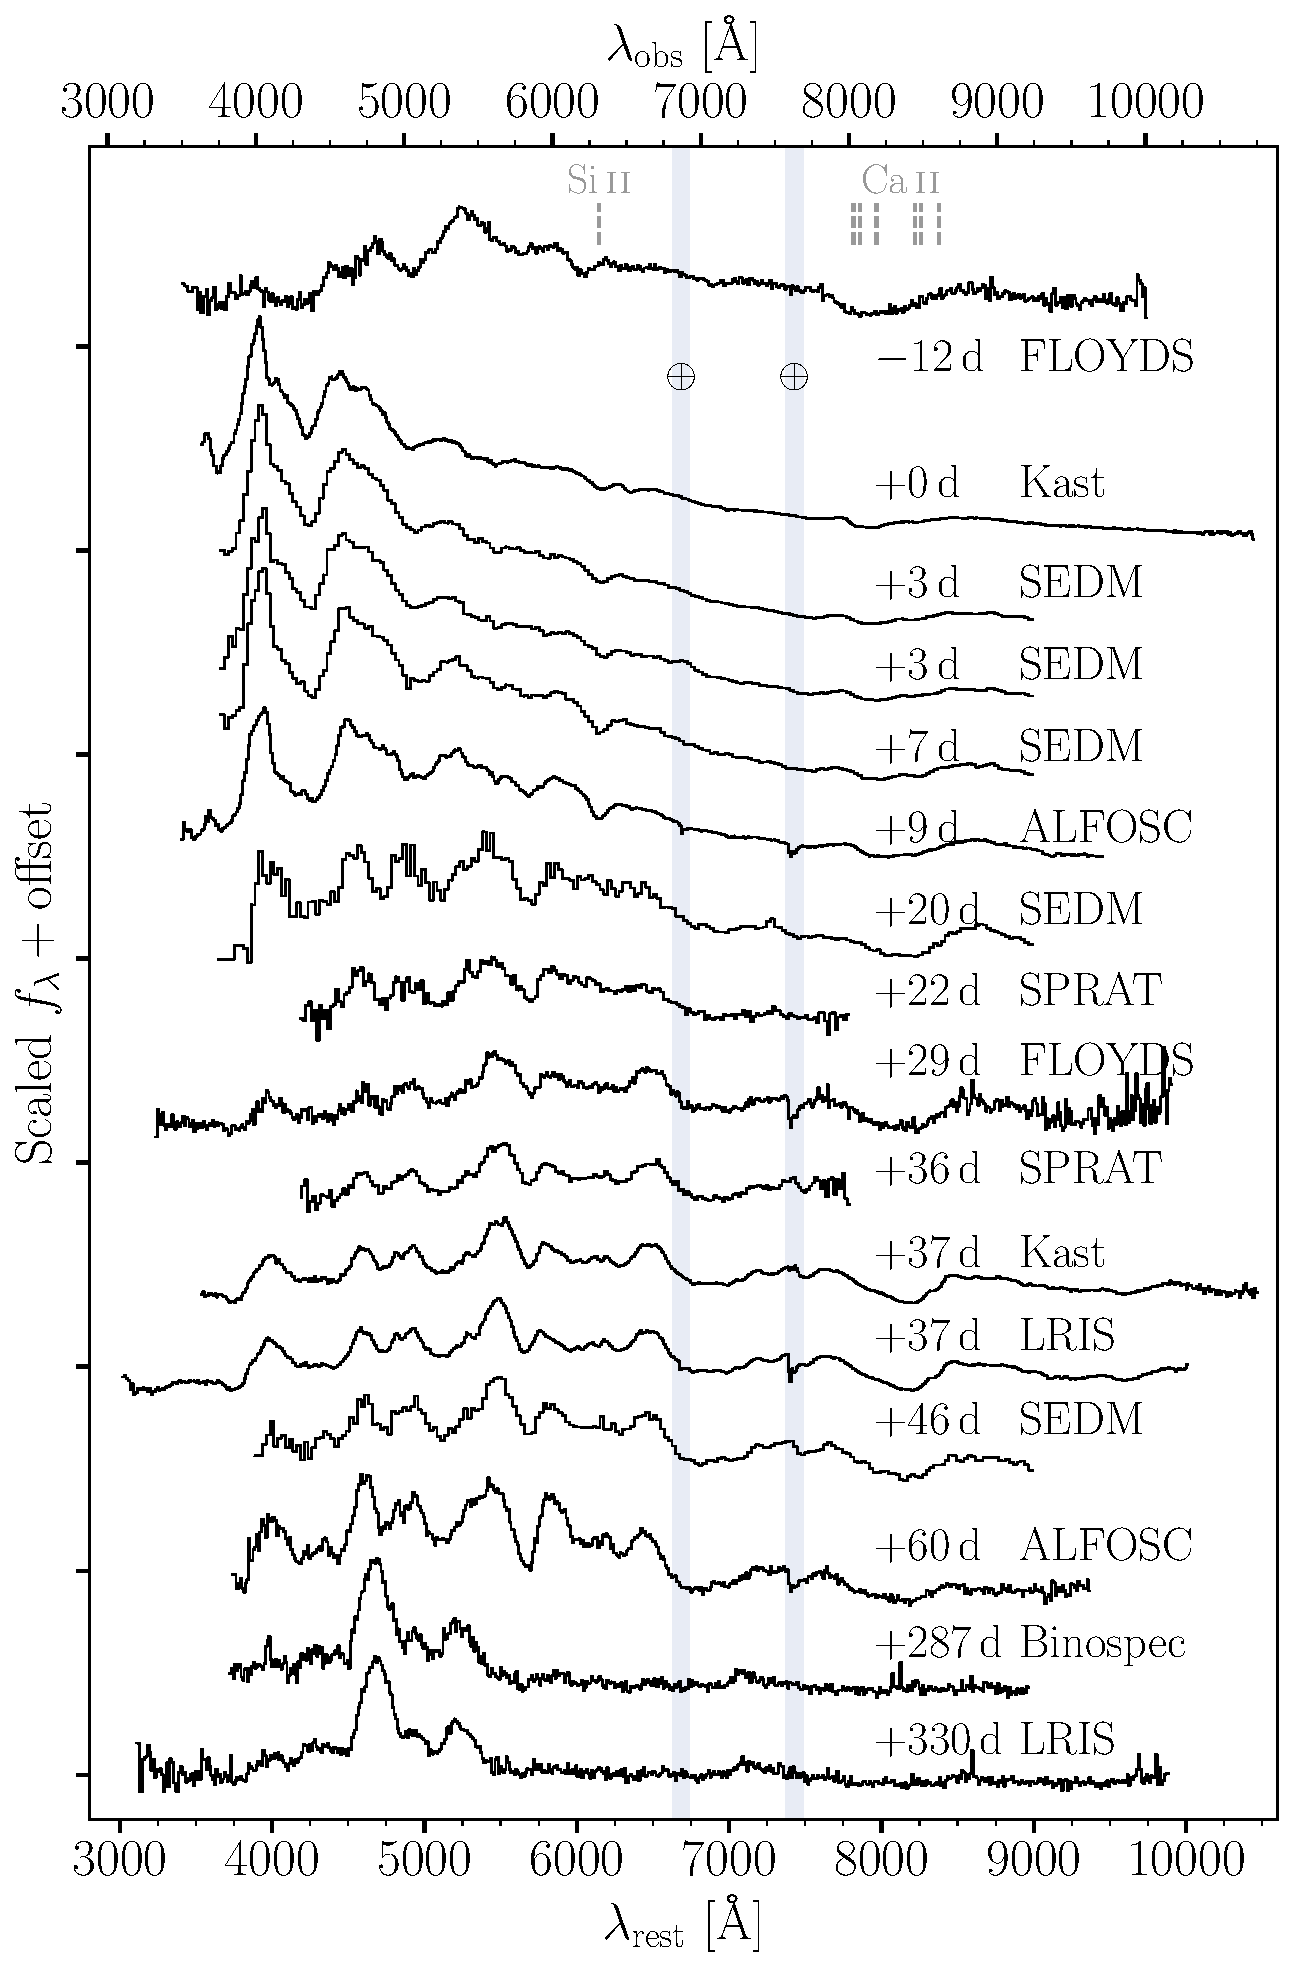
\includegraphics[width=\linewidth]{SN2022joj_spectral_sequence.pdf}
    \caption{Optical spectral sequence of \sn. Rest-frame phases (days) relative to the $B$-band peak and instruments used are posted next to each spectrum. Spectra have been corrected for $E(B-V)_\mathrm{MW} = 0.04$\,mag and are shown in gray. The black lines are binned spectra with a bin size of 10\,\AA, except for the SEDM spectra, whose resolution is lower than the bin size. The corresponding wavelengths of the \ion{Si}{2} $\lambda$6355 line (with an expansion velocity of 10,000\,\kms) and the \ion{Ca}{2} IRT (with expansion velocities of both 10,000\,\kms and 25,000\,\kms) are marked by the vertical dashed lines.}
    \label{fig:spec_seq}
\end{figure}

\begin{deluxetable}{lrcccc}
\tabletypesize{\scriptsize}
\tablewidth{0pt}
\tablecaption{Spectroscopic observations of \sn\label{tab:spectra} and the host galaxy.}
\tablehead{
\colhead{$t_\mathrm{obs}$} &
\colhead{Phase} &
\colhead{Telescope/} &
\colhead{$R$} &
\colhead{Range} &
\colhead{Airmass} \\
\colhead{(MJD)} &
\colhead{(days)} &
\colhead{Instrument} &
\colhead{$(\lambda/\Delta\lambda)$} &
\colhead{(\AA)} & 
\colhead{}
}
\startdata
58,976.42 &  $-$9.7 & P60/SEDM & 100 & 3770--9220 & 1.23\\
58,982.12 & $-$4.2 & NOT/ALFOSC & 360 & 4000--9620 & 1.17\\
58,990.43 &  $+$3.9 & P60/SEDM & 100 & 3770--9220 &  1.23\\
58,997.44 & $+$10.7 & P60/SEDM & 100 & 3770--9220 &  1.29\\
58,998.41 & $+$11.6 & Shane/Kast & 750 & 3620--10720 & 1.28\\ % 300/7500, 4.60 A/pix, FWHM ~ 10 A
59,008.41 & $+$21.3 & P60/SEDM & 100 & 3770--9220 & 1.28\\
59,009.45 & $+$22.4 & Gemini-N/GNIRS & 1800 & 8230--25150 &1.07\\
59,010.40 & $+$23.3 & P200/DBSP & 700 & 3200--9500 &  1.27\\
59,023.58 & $+$36.1 & Keck I/LRIS & 1100 & 3200--10250 & 2.04\\
59,107.29 & $+$117.3 & Keck I/LRIS & 1100 & 3200--10250 & 1.31\\
59,143.26 & $+$152.2 & Keck I/LRIS & 1100 & 3200--10250 & 2.16\\
59,669.60 & host & Keck II/DEIMOS & 2100 & 4500--8700 & 1.14\\ % 600ZD, blaze wavelength 7500 A, FWHM resolution 3.5 A
\enddata
\tablecomments{Phase is measured relative to the $r_\mathrm{ZTF}$-band peak in the rest frame of the host galaxy. The resolution $R$ is reported for the central region of the spectrum.}
\label{tab:spec}
\end{deluxetable}


\begin{figure*}
    \centering
    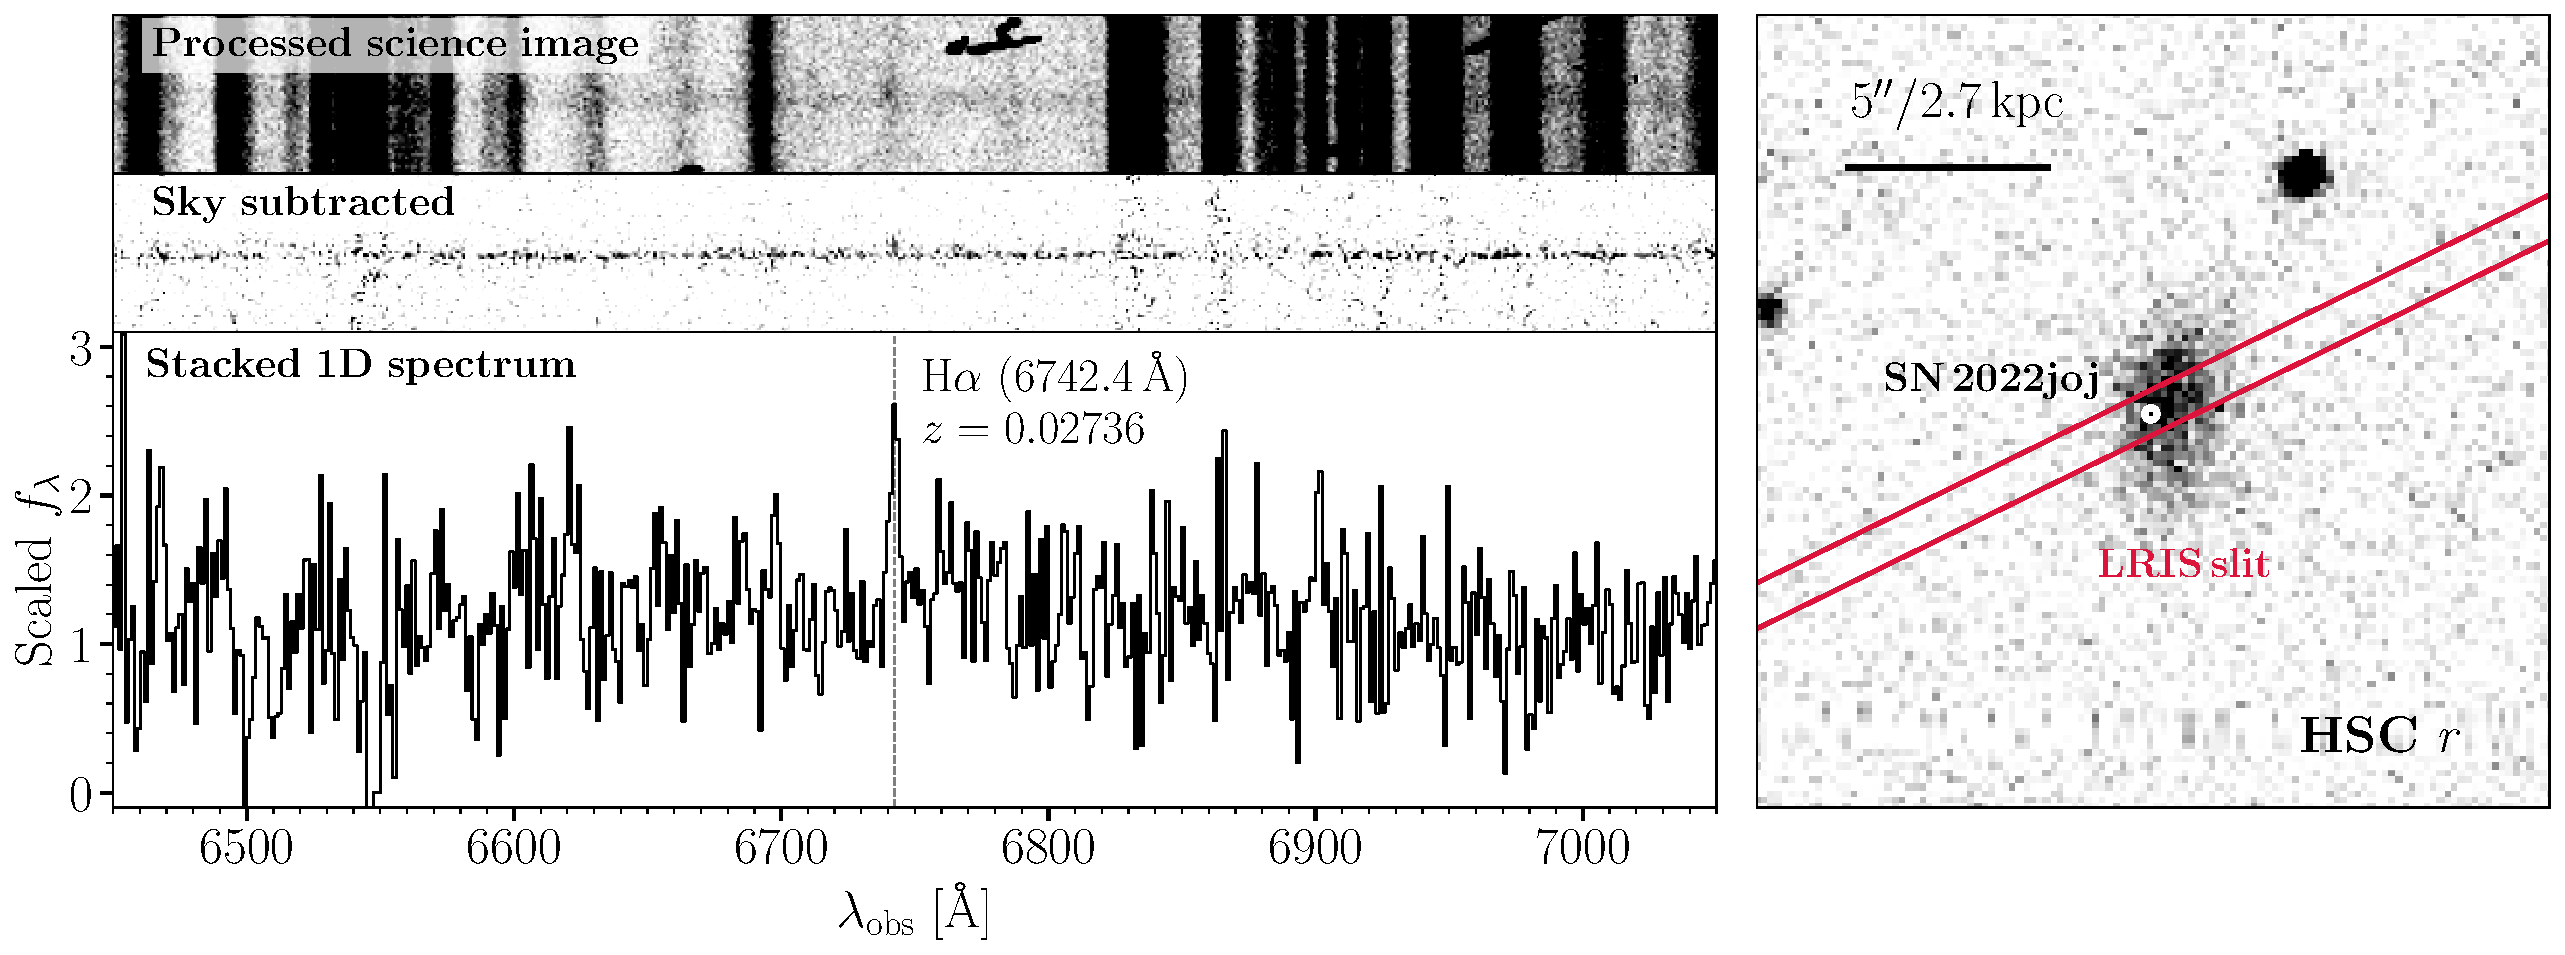
\includegraphics[width=\linewidth]{host_spec.pdf}
    \caption{The LRIS spectra reveal the H$\alpha$ emission line from the host galaxy at 6742.4\,\AA, corresponding to a redshift $z=0.02736$.}
    \label{fig:host_spec}
\end{figure*}

\section{Analysis} \label{sec:analysis}

\subsection{Optical Spectral Properties}
\begin{figure*}
    \centering
    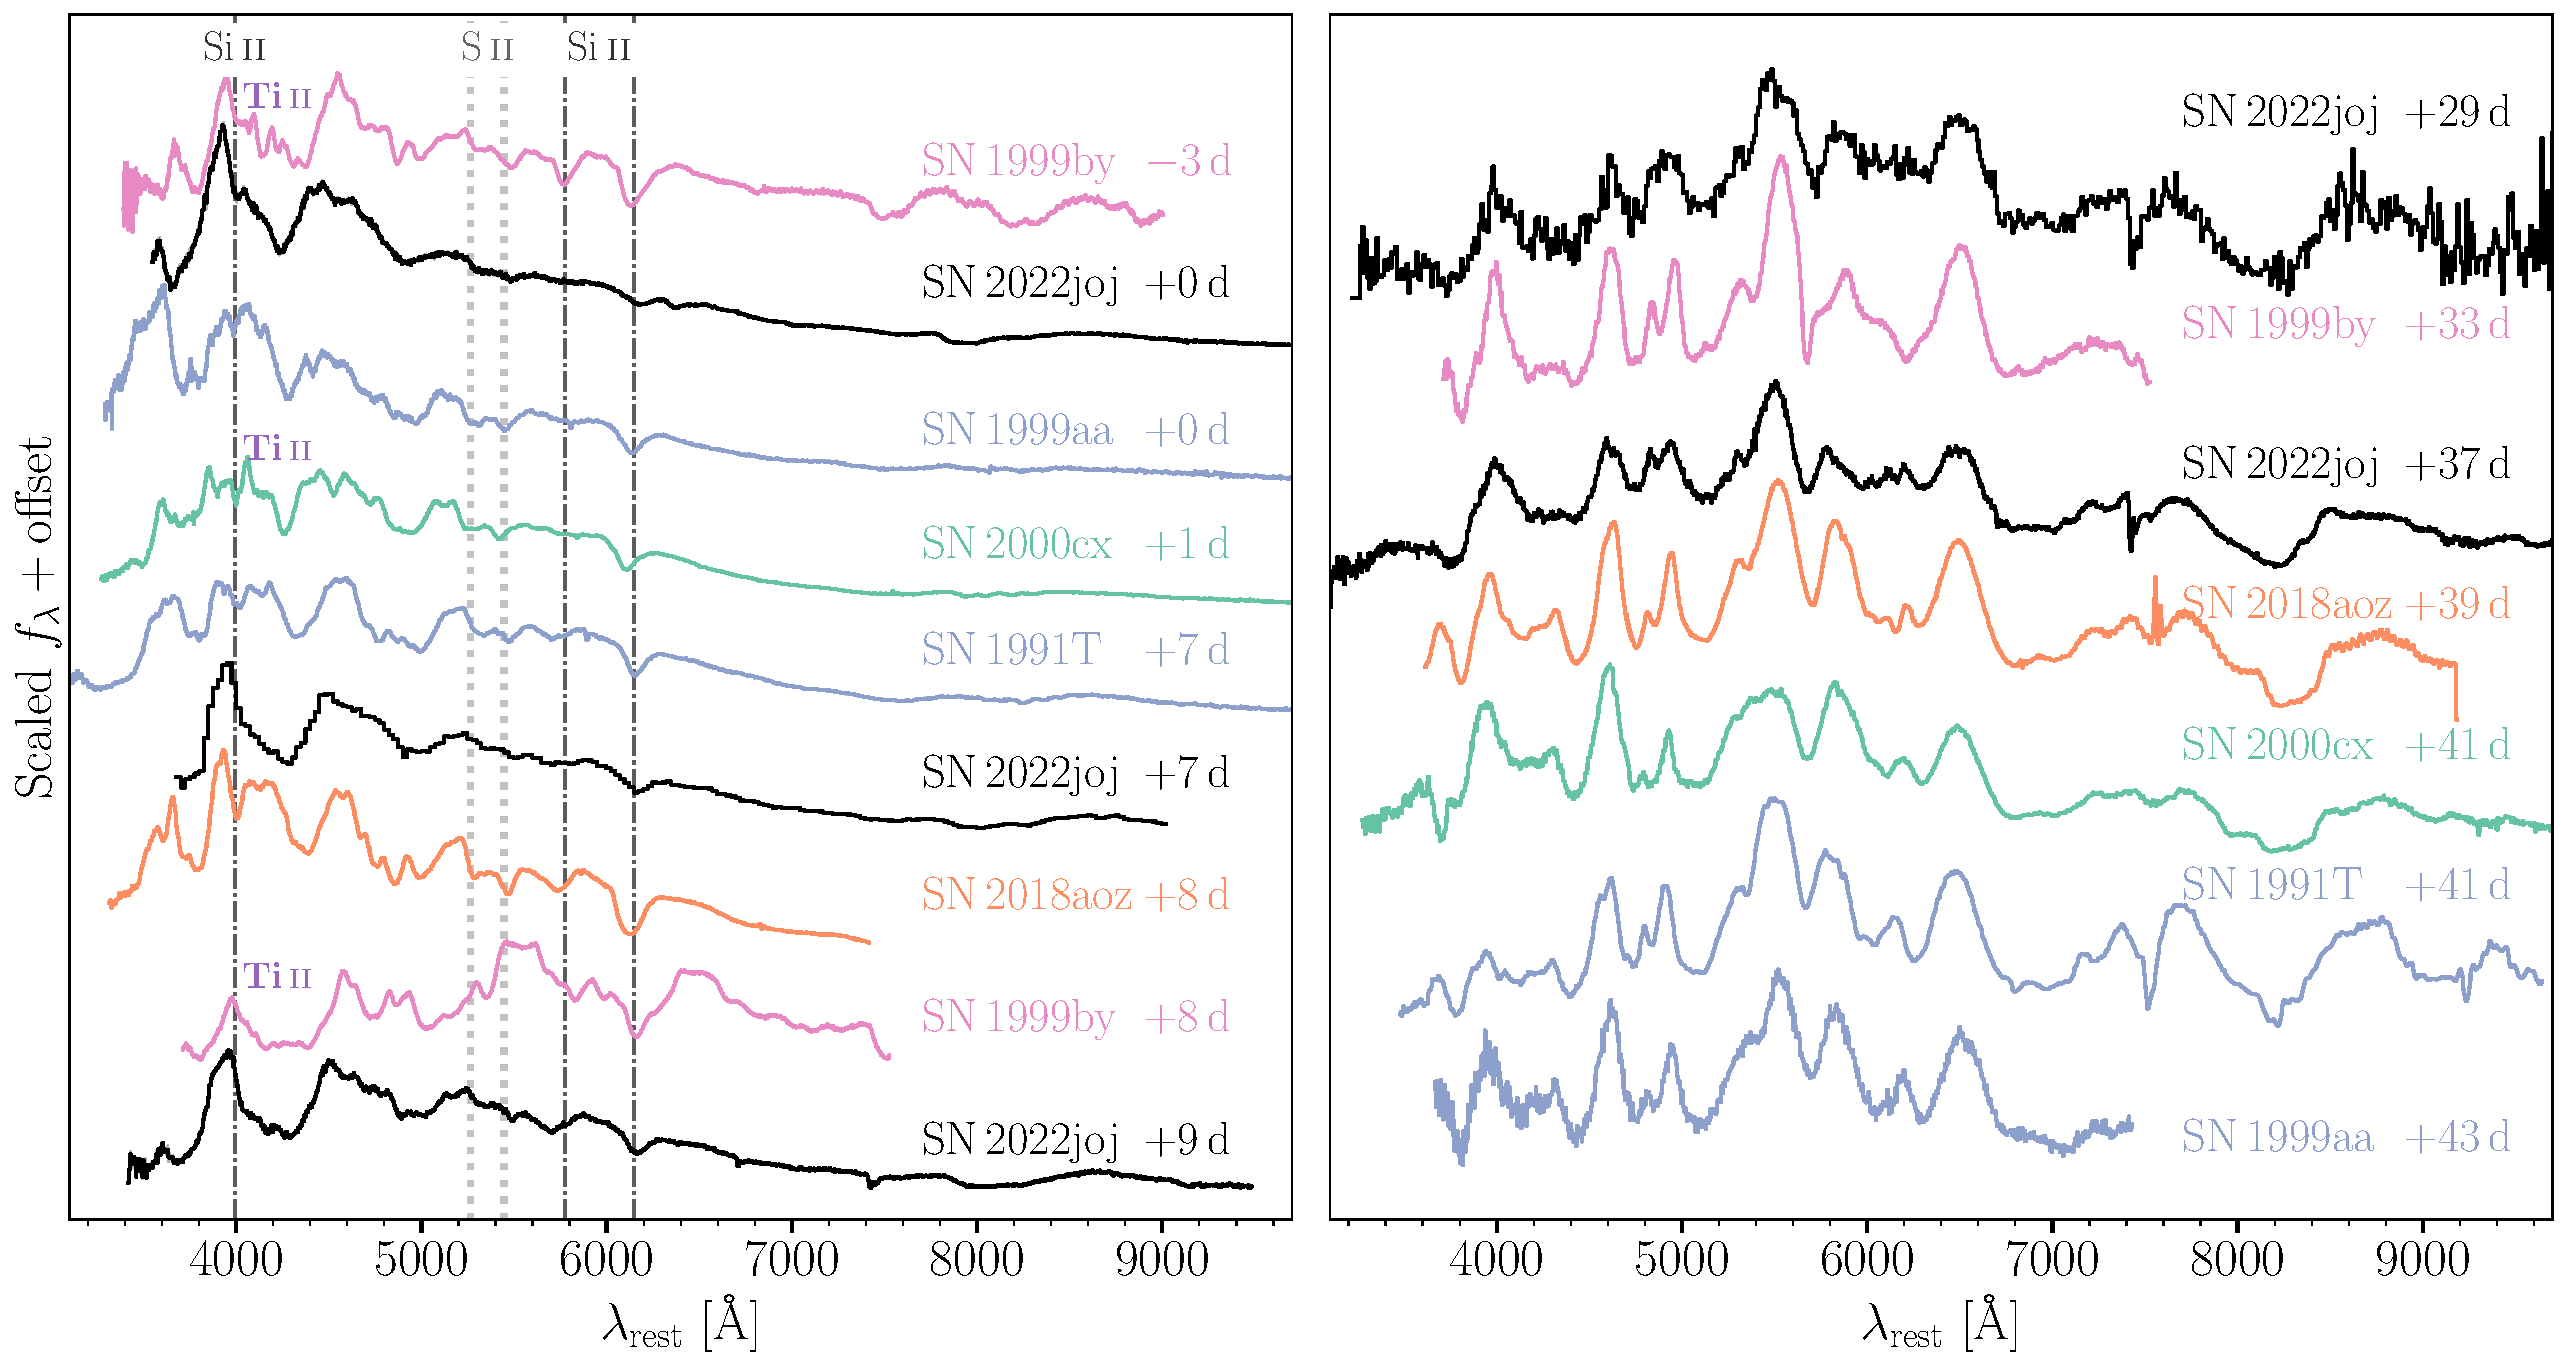
\includegraphics[width=\linewidth]{spec_comp.pdf}
    \caption{Optical spectral sequence of \sn.}
    \label{fig:spec_comp}
\end{figure*}

\begin{figure*}
    \centering
    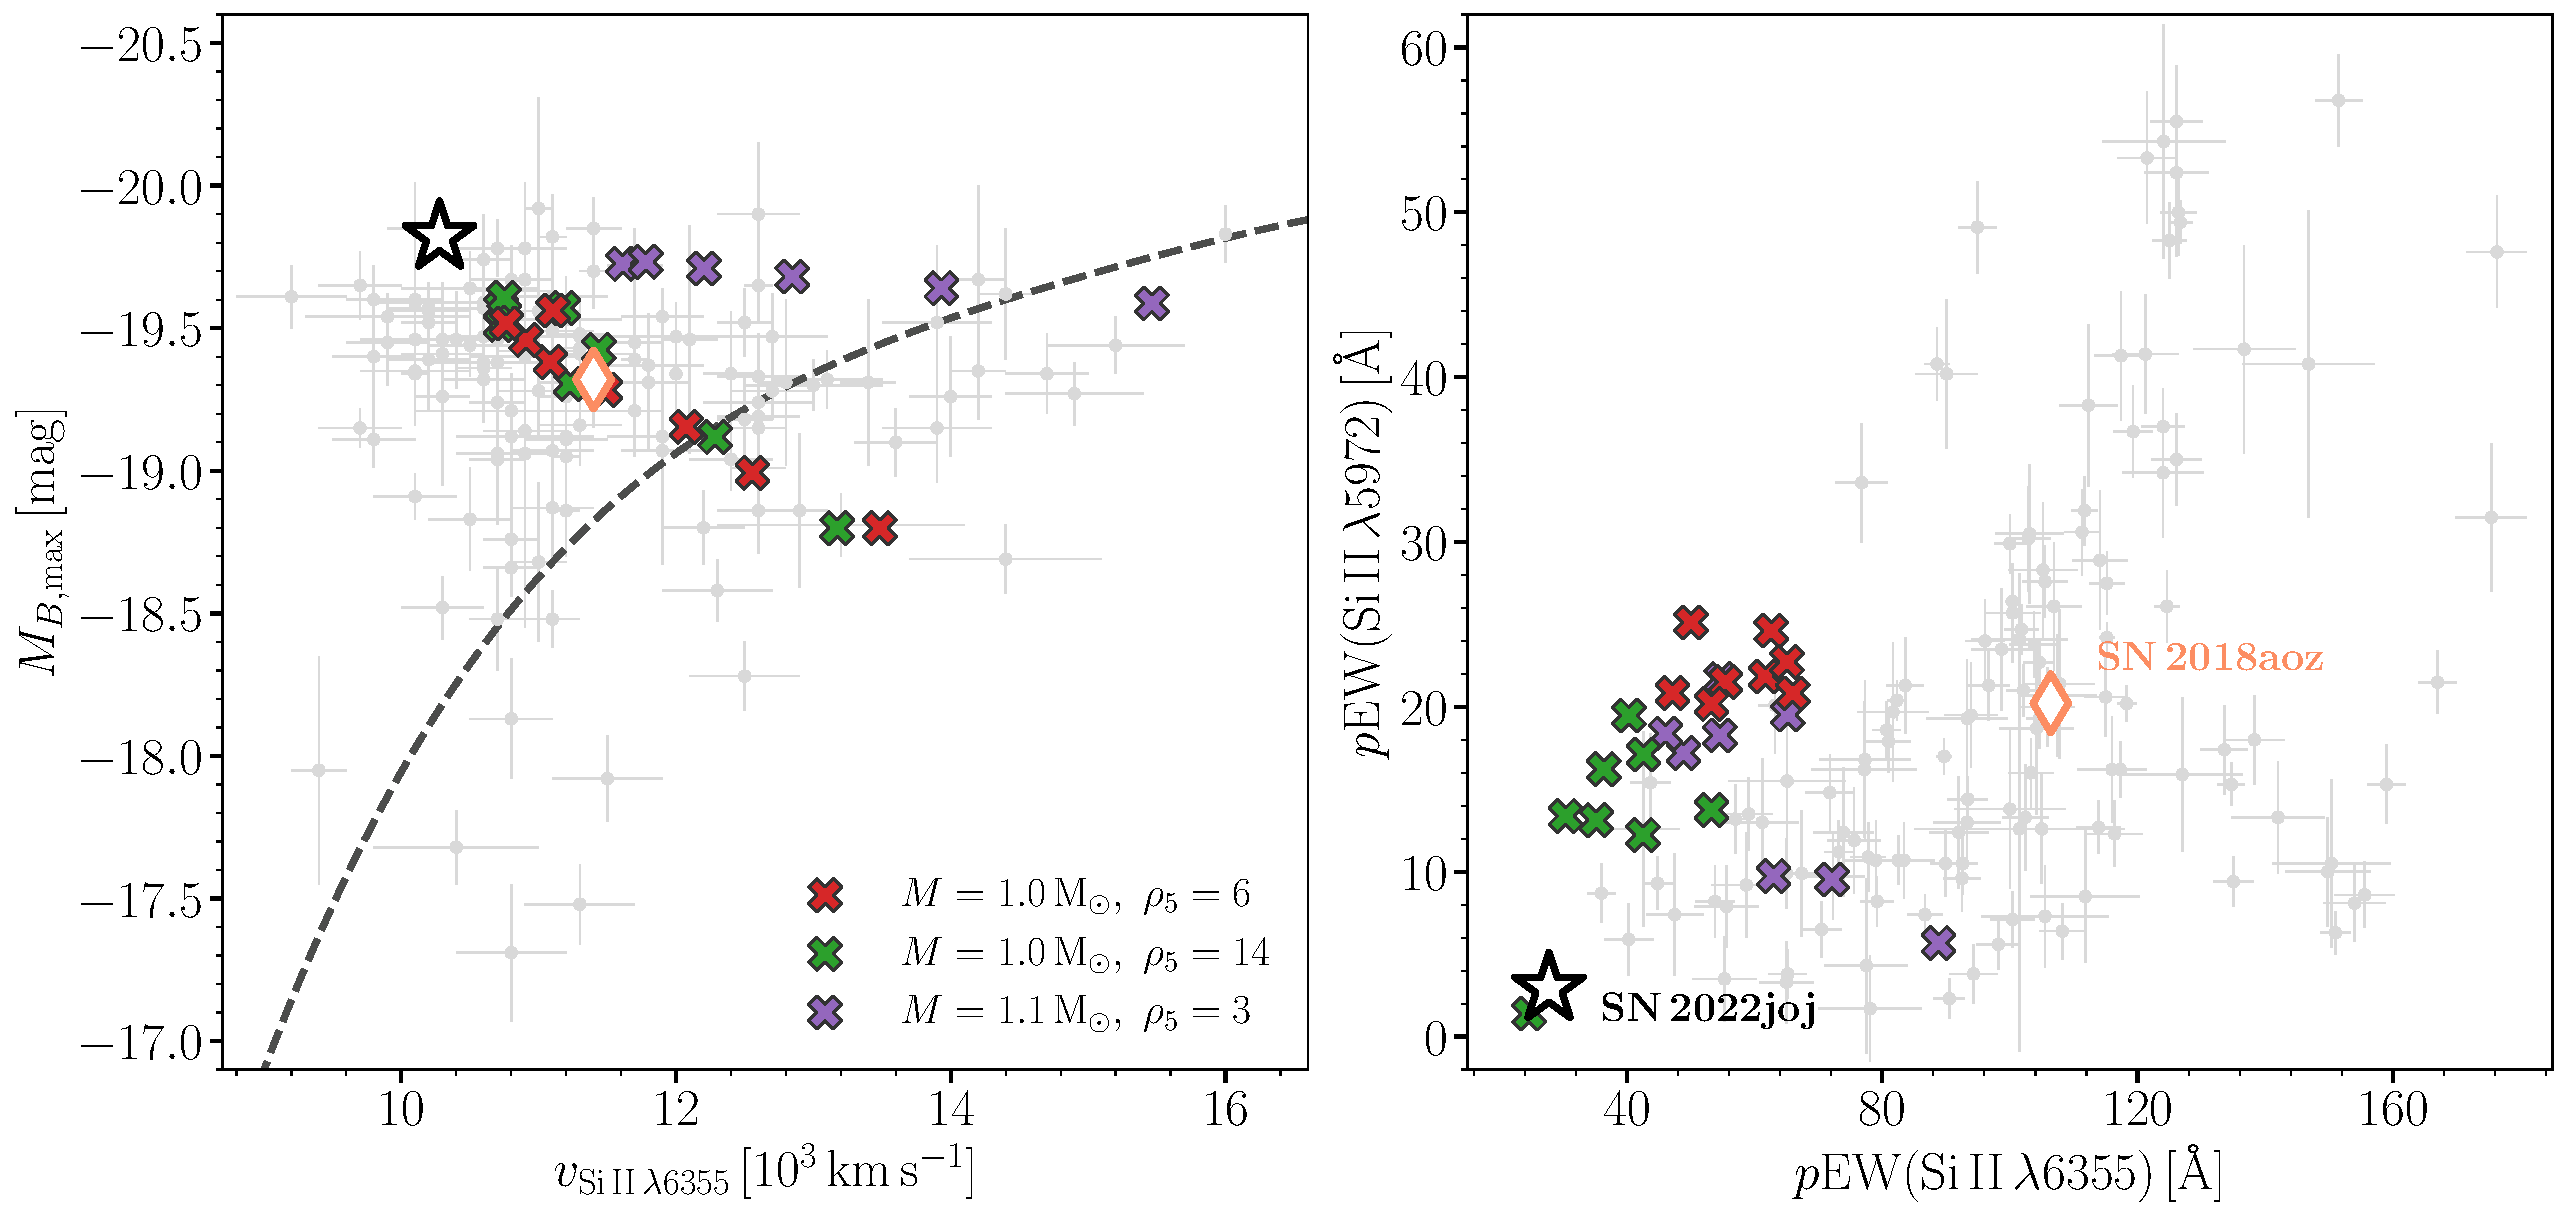
\includegraphics[width=\linewidth]{phase_space.pdf}
    \caption{\sn\ as a SN\,Ia in the shallow-silicon class.}
    \label{fig:phase_space}
\end{figure*}

\section{Discussion} \label{sec:discussion}
\subsection{Models} \label{sec:model}
\begin{figure*}
    \centering
    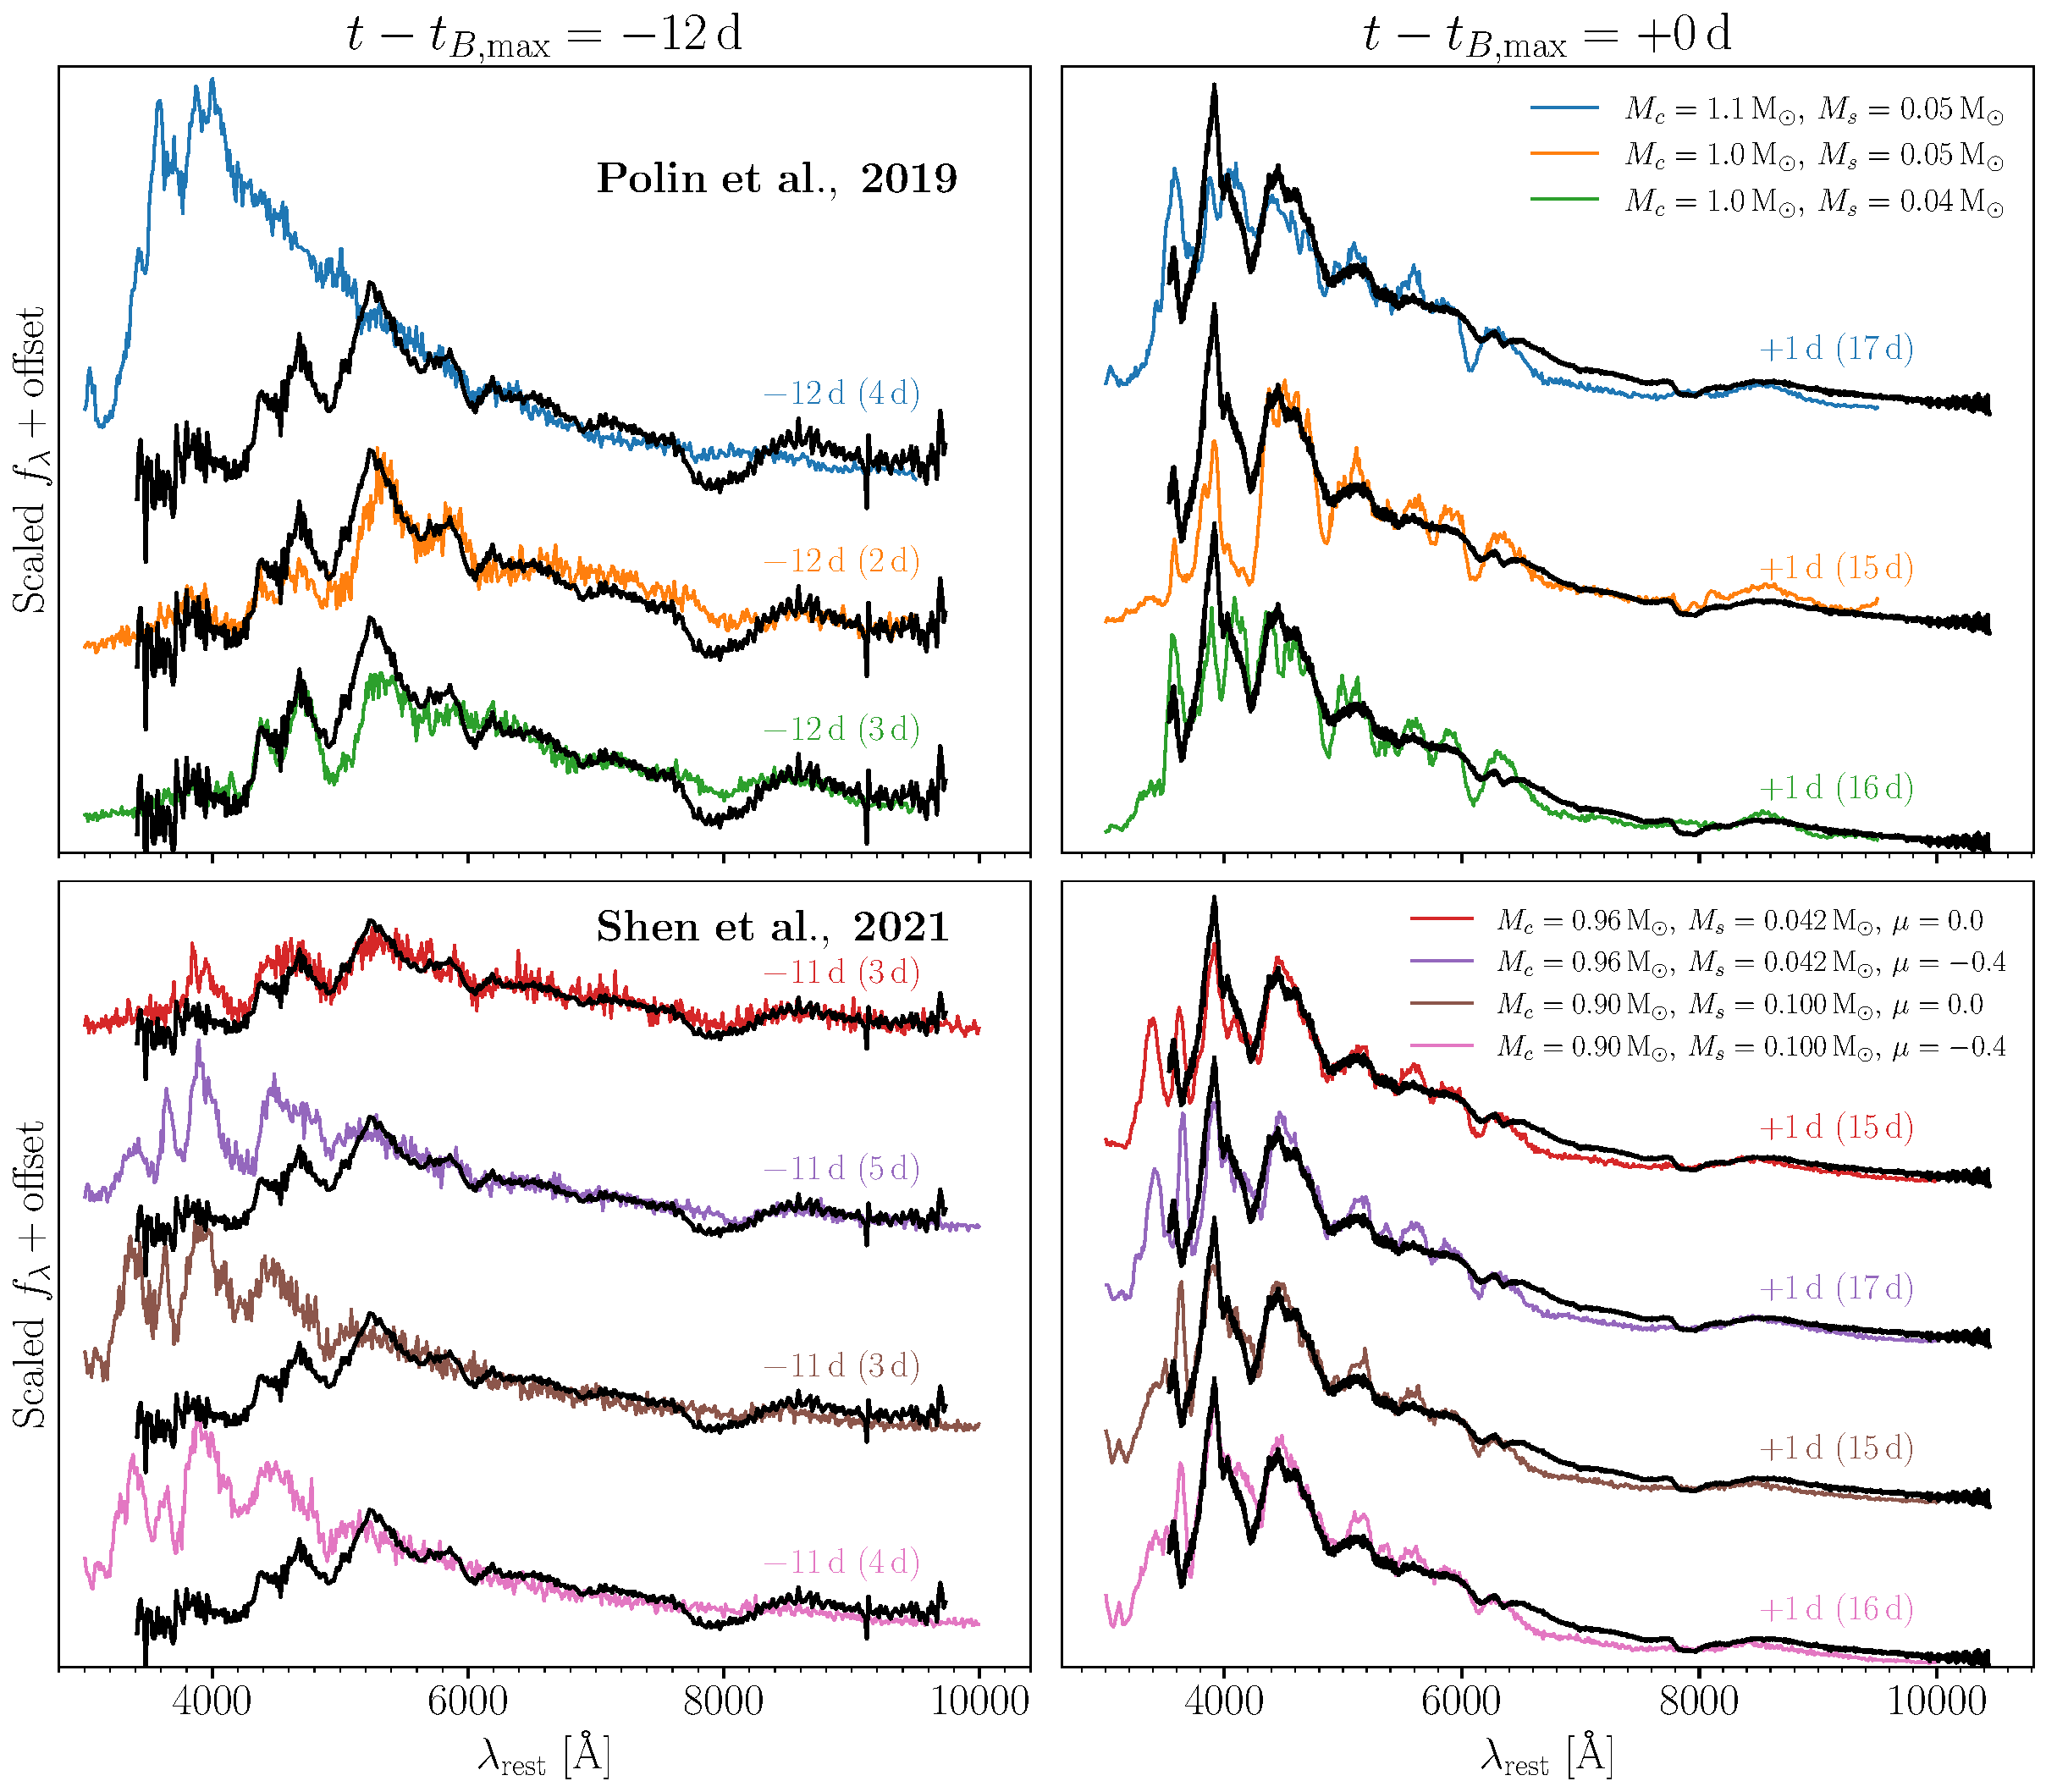
\includegraphics[width=\linewidth]{model_comparison_spec.pdf}
    \caption{\sn\ v.s. DDet models.}
    \label{fig:model_spec}
\end{figure*}

\subsection{Nebular-phase Spectra}
\begin{itemize}
    \item weak emission in the 7300 complex compared to normal SNe\,Ia -- similar to 91T-like events
    \item Blueshifted [\ion{Fe}{2}] 7300 features ($\sim$$-2.21\pm0.33\mathrm{\,km\,s^{-1}}$ in the Binospec spectrum; $\sim$$-1.24\pm0.42\mathrm{\,km\,s^{-1}}$ in the LRIS spectrum), consistent with low-\ion{Si}{2}-velocity SNe Ia
    \item No evidence for [\ion{Ni}{2}] $\lambda\lambda$7378, 7412 or [\ion{Ca}{2}] $\lambda\lambda$7291, 7323 -- 3-$\sigma$ upper limit for $M_\mathrm{Fe}/M_\mathrm{Ni}$ is 0.05 (techniques adopted from \citet{Maguire_2018}), consistent with sub-\Mch\ DDet scenario?
\end{itemize}
\section{Conclusions} \label{sec:conclusion}

%\begin{acknowledgements}

% \noindent {We thank the anonymous referee for a thoughtful and detailed report.} We thank Eddie Schlafly and Dustin Lang for suggesting photometry from DESI Legacy Imaging Surveys in SED fitting. We are grateful to Aishwarya Dahiwale, Jillian Rastinejad, and Yuhan Yao for the high-quality spectra they obtained. We also appreciate the excellent assistance of the staffs of the various observatories where data were obtained. K.D. acknowledges support from NASA through the NASA Hubble Fellowship grant \#HST-HF2-51477.001 awarded by the Space Telescope Science Institute, which is operated by the Association of Universities for Research in Astronomy, Inc., for NASA, under contract NAS5-26555. A.V.F. is grateful for financial support from the Christopher R. Redlich Fund and many other individual donors. K.M. is funded by the EU H2020 ERC grant No. 758638. S.S. acknowledges support from the G.R.E.A.T research environment, funded by {\em Vetenskapsr\aa det}, the Swedish Research Council, project number 2016-06012. This work was also supported by the GROWTH project \citep{Kasliwal2019} funded by the National Science Foundation (NSF) under grant 1545949.

% This work is based on observations obtained with the Samuel Oschin Telescope 48-inch and the 60-inch Telescope at the Palomar Observatory as part of the Zwicky Transient Facility project. ZTF is supported by the National Science Foundation under Grant No. AST-1440341 and a collaboration including Caltech, IPAC, the Weizmann Institute of Science, the Oskar Klein Center at Stockholm University, the University of Maryland, the University of Washington, Deutsches Elektronen-Synchrotron and Humboldt University, Los Alamos National Laboratories, the TANGO Consortium of Taiwan, the University of Wisconsin at Milwaukee, and Lawrence Berkeley National Laboratories. Operations are conducted by COO, IPAC, and UW. 
% SED Machine is based upon work supported by the National Science Foundation under Grant No.\ 1106171.

% This work is also based on observations made with the Nordic Optical Telescope, owned in collaboration by the University of Turku and Aarhus University, and operated jointly by Aarhus University, the University of Turku and the University of Oslo, representing Denmark, Finland and Norway, the University of Iceland and Stockholm University at the Observatorio del Roque de los Muchachos, La Palma, Spain, of the Instituto de Astrofisica de Canarias.

% A major upgrade of the Kast spectrograph on the Shane 3\,m telescope at Lick Observatory, led by Brad Holden, was made possible through gifts from the Heising-Simons Foundation, William and Marina Kast, and the University of California Observatories. Research at Lick Observatory is partially supported by a generous gift from Google. The W. M. Keck Observatory is operated as a scientific partnership among the California Institute of Technology, the University of California and NASA; the observatory was made possible by the generous financial support of the W. M. Keck Foundation. {W. M. Keck Observatory access was supported by Northwestern University and the Center for Interdisciplinary Exploration and Research in Astrophysics (CIERA).}

%\end{acknowledgements}

\facility{PO:1.2m (ZTF), PO:1.5m (SEDM), FTN (FLOYDS), FTS (FLOYDS), NOT (ALFOSC), Liverpool:2m (SPRAT), Keck:I (LRIS), MMT (Binospec).}
\software{\texttt{astropy} \citep{Astropy_2013, Astropy_2018}, \texttt{CASTRO} \citep{Almgren_Castro_2010}, \texttt{dynesty} \citep{Speagle_dynesty_2020}, \texttt{LAMBDAR} \citep{Wright2016a}, \texttt{matplotlib} \citep{Matplotlib_2007}, \texttt{prospector} \citep{Johnson_prospector_2021}, \texttt{PypeIt} \citep{pypeit:zenodo}, \texttt{pysedm} \citep{Rigault_pysedm_2019}, \texttt{Python-FSPS} \citep{Conroy_2009,Conroy_2010}, \texttt{scipy} \citep{Scipy_2020}, \texttt{seaborn} \citep{Waskom_seaborn_2021}, \texttt{SEDONA} \citep{Kasen_Sedona_2006}.}


\bibliography{SN2022joj, software, telescope}
\bibliographystyle{aasjournal}

%% This command is needed to show the entire author+affiliation list when
%% the collaboration and author truncation commands are used.  It has to
%% go at the end of the manuscript.
%\allauthors

%% Include this line if you are using the \added, \replaced, \deleted
%% commands to see a summary list of all changes at the end of the article.
%\listofchanges

\end{CJK*}
\end{document}

% End of file `sample631.tex'.
